\documentclass[tikz, border=2pt]{standalone}

\usepackage{amsmath,amssymb}
\usepackage{pgfplots}
\pgfplotsset{compat=1.18}
\usetikzlibrary{arrows.meta}
\usepackage{xcolor}

\definecolor{utnblue}{RGB}{0, 51, 102}

\begin{document}
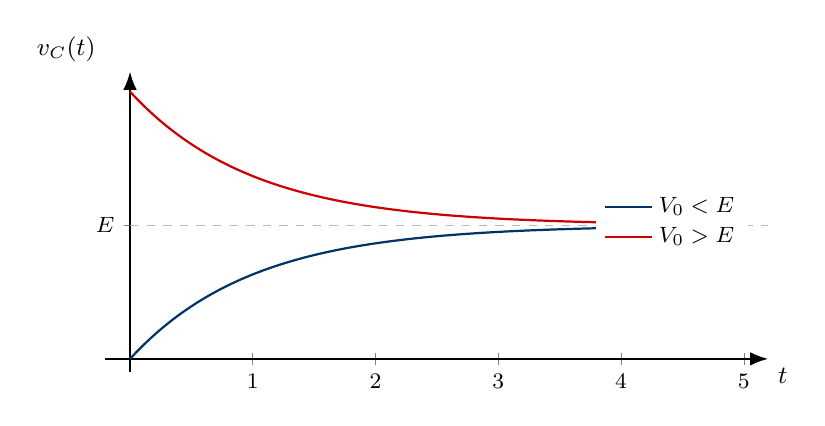
\begin{tikzpicture}[>=Latex, font=\small]
\begin{axis}[
    axis lines=middle,
    axis line style={->, thick, black},
    width=10cm, height=5.4cm,
    xlabel={$t$}, ylabel={$v_C(t)$},
    xlabel style={anchor=north west},
    ylabel style={rotate=0, anchor=south east, at={(axis description cs:0,1)}},
    xmin=-0.2, xmax=5.2,
    ymin=-0.1, ymax=2.15,
    ytick={1}, yticklabels={$E$},
    yticklabel style={font=\footnotesize},
    xticklabel style={font=\footnotesize},
    samples=200, domain=0:5,
    clip=false,
    legend style={draw=none, at={(0.97,0.5)}, anchor=east, font=\footnotesize},
]
    % asintota en E
    \addplot[gray!55, thin, dashed, forget plot] coordinates {(0,1) (5.2,1)};
    % V0 < E : sube hacia E   (V0 = 0)
    \addplot[utnblue, thick] {1 - exp(-x)};
    \addlegendentry{$V_0<E$}
    % V0 > E : baja hacia E    (V0 = 2)
    \addplot[red!80!black, thick] {1 + exp(-x)};
    \addlegendentry{$V_0>E$}
\end{axis}
\end{tikzpicture}
\end{document}
